% =====================================================================
%  Front and back cover, A4, same page size as the book.
%
%  Division of labour: the artwork in art/ contains no letters at all (see
%  figures/make_covers.py), so every word here is typeset. That is deliberate --
%  an image model asked to write a title produces a plausible title with one
%  letter out of place, and asked to write an identifier it invents one.
%
%  There is no ISBN, no ISSN, no DOI and no barcode on either page, on request.
%
%  Build: latexmk -pdf cover.tex   (run before the main file; the book includes
%  the result with 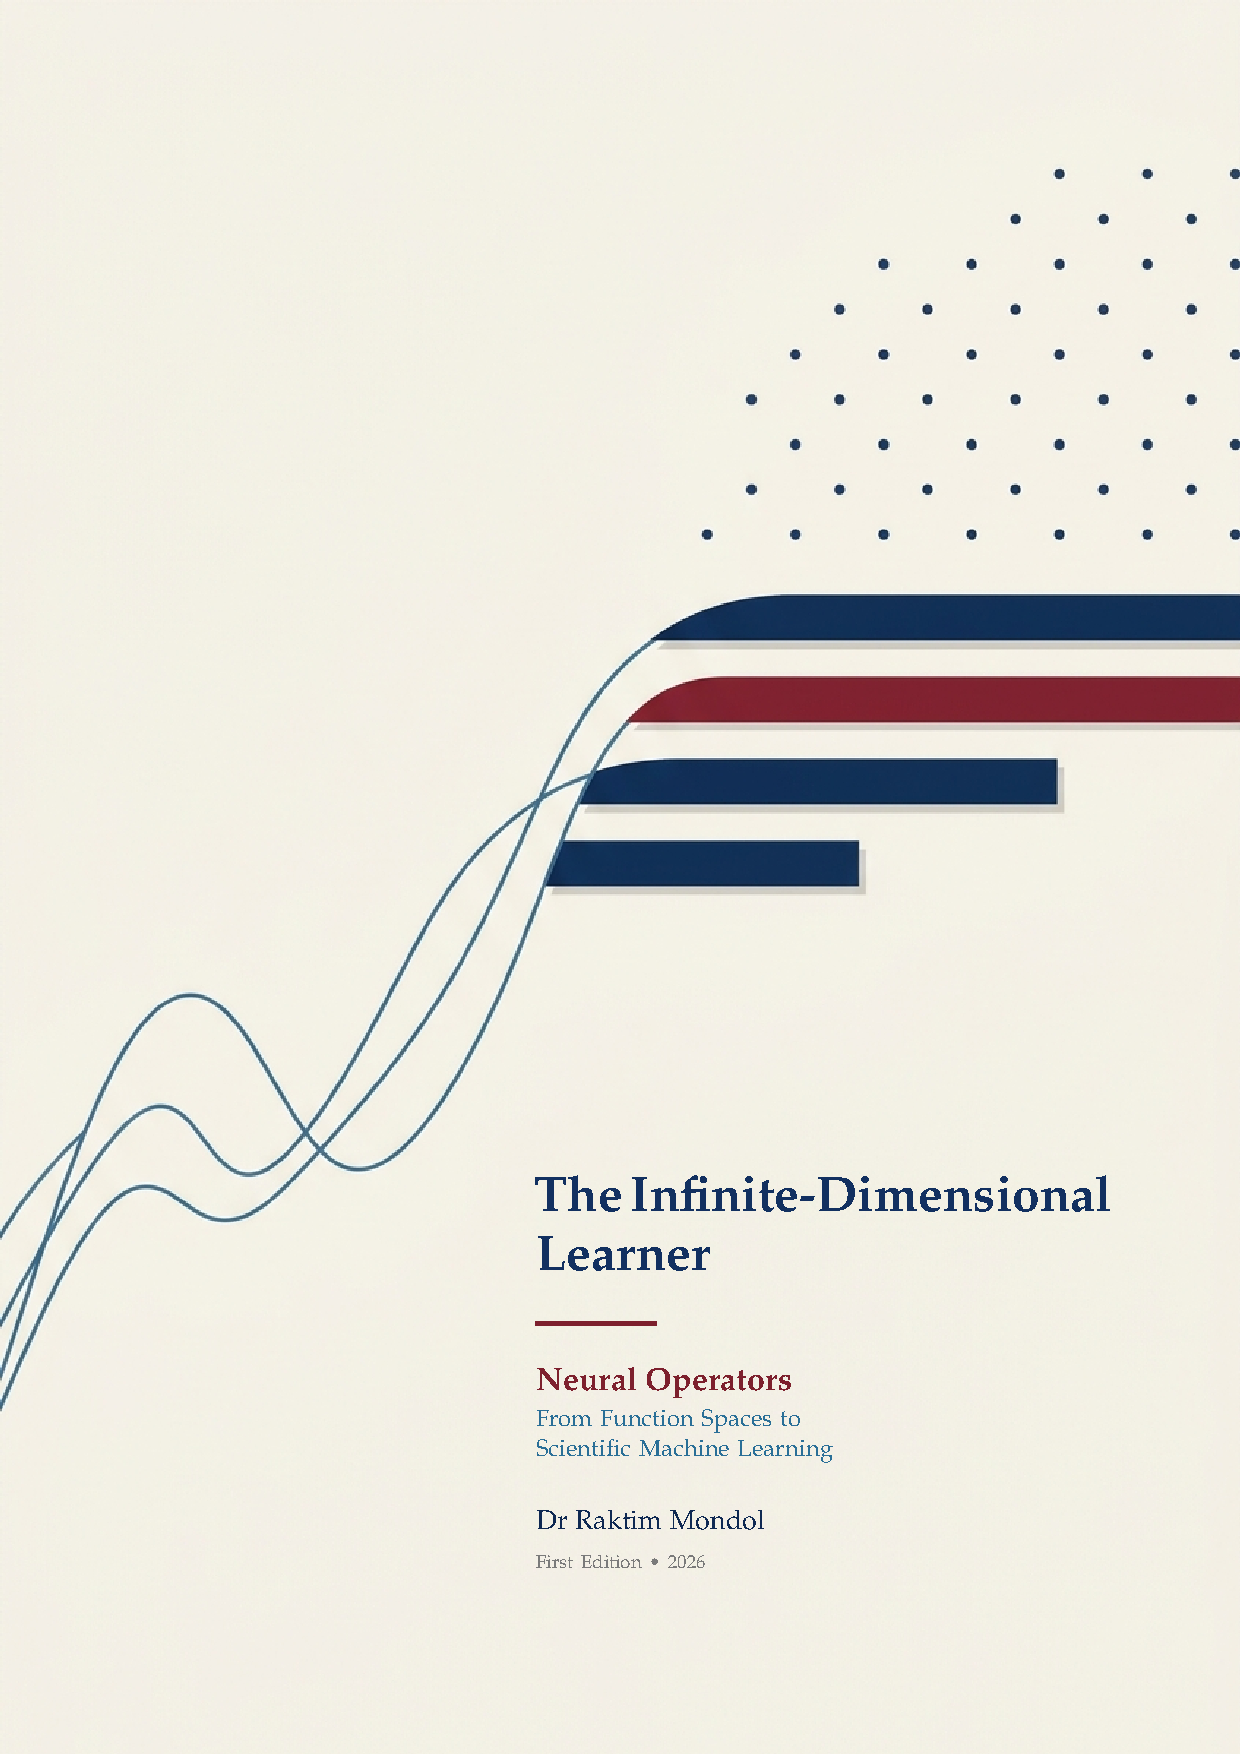
\includepdf{covers/cover.pdf})
% =====================================================================
\documentclass[a4paper,11pt]{article}
\usepackage[utf8]{inputenc}
\usepackage[T1]{fontenc}
\usepackage{mathpazo}
\usepackage{amssymb}
\usepackage[dvipsnames]{xcolor}
\usepackage{graphicx}
\usepackage{tikz}
\usepackage{microtype}
\usepackage[a4paper,margin=0pt]{geometry}

\definecolor{primary}{RGB}{18,48,96}
\definecolor{secondary}{RGB}{125,32,45}
\definecolor{accent}{RGB}{42,111,151}

\pagestyle{empty}
\graphicspath{{art/}}

% Text pockets are chosen from where the two compositions have no ink. Measured
% off the cropped rasters: on the front nothing sits right of 42% below 55% of
% the page height; on the back nothing sits right of 46% below 60%, and the
% whole upper-left quadrant is clear down to 55%.
\newcommand{\margin}{56pt}

\begin{document}

% ------------------------------------------------------------- front cover
\begin{tikzpicture}[remember picture,overlay]
\node[inner sep=0pt,anchor=north west] at (current page.north west)
  {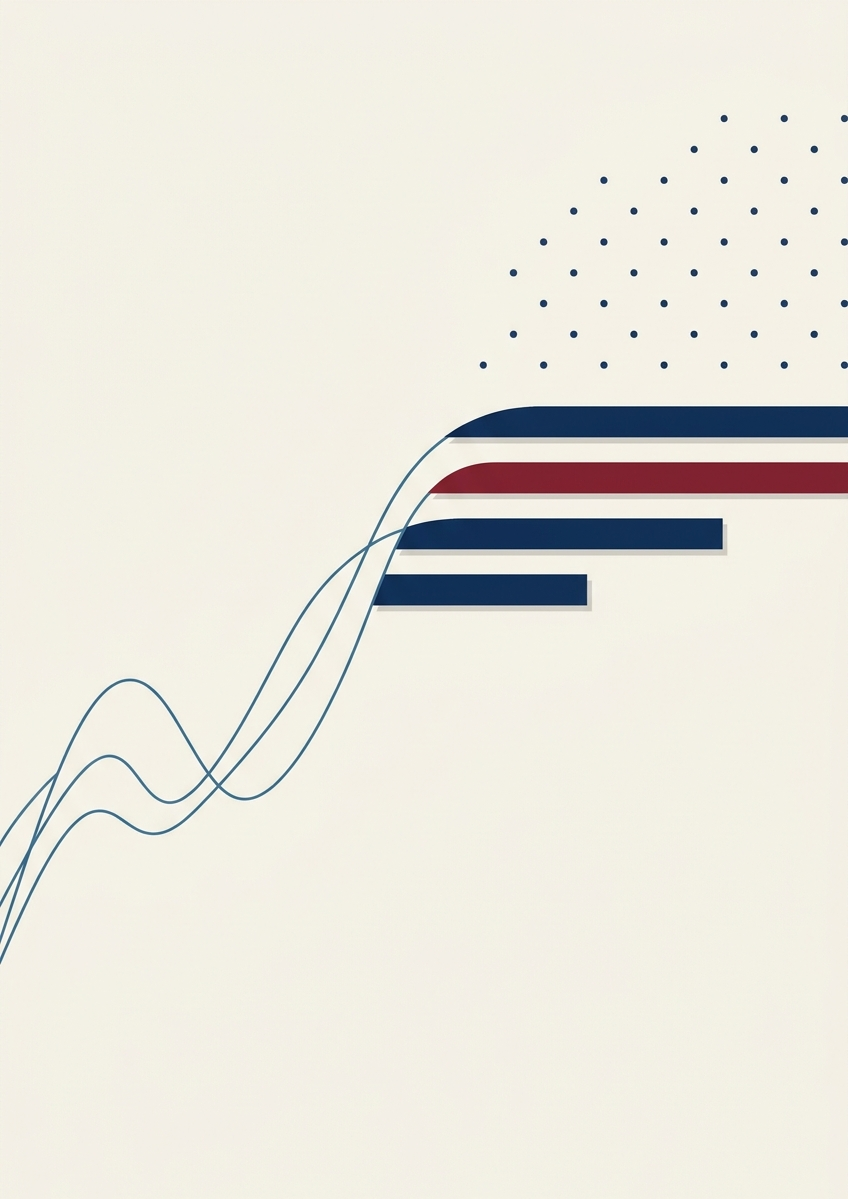
\includegraphics[width=\paperwidth,height=\paperheight]{front_a4}};

% "The Infinite-Dimensional" is 278 pt at 24 pt and 313 pt at 27 pt. The block is
% 284 pt wide because that is what the pocket allows with its left edge kept on the
% 43 % line, where the artwork's bands begin, so the title is set at 24 pt and the
% compound is broken by hand rather than left to wrap.
\node[inner sep=0pt,anchor=north west,text width=284pt,align=left]
  at ([xshift=258pt,yshift=-566pt]current page.north west)
  {\parindent=0pt
   {\fontsize{24}{28.5}\selectfont\bfseries\color{primary} The Infinite-Dimensional\\
    Learner\par}
   \vspace{13pt}
   {\color{secondary}\rule{58pt}{2.2pt}\par}
   \vspace{12pt}
   {\fontsize{15.5}{19}\selectfont\bfseries\color{secondary} Neural Operators\par}
   \vspace{3pt}
   {\fontsize{11.5}{14.5}\selectfont\color{accent} From Function Spaces to\\
    Scientific Machine Learning\par}
   \vspace{19pt}
   {\fontsize{13}{16}\selectfont\color{primary!85!black} Dr Raktim Mondol\par}
   \vspace{7pt}
   {\fontsize{9}{12}\selectfont\color{black!52} First Edition \textbullet{} 2026\par}};
\end{tikzpicture}
\clearpage

% -------------------------------------------------------------- back cover
\begin{tikzpicture}[remember picture,overlay]
\node[inner sep=0pt,anchor=north west] at (current page.north west)
  {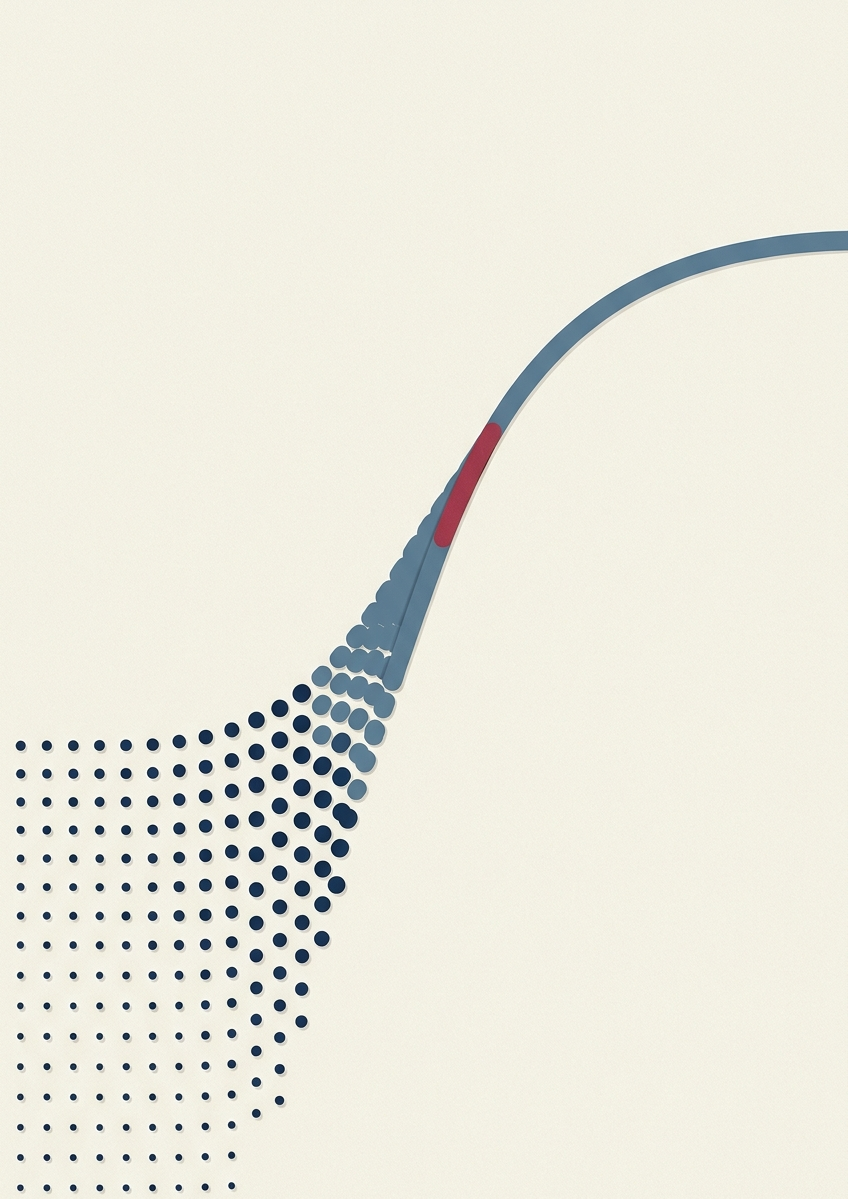
\includegraphics[width=\paperwidth,height=\paperheight]{back_a4}};

\node[inner sep=0pt,anchor=north west,text width=214pt,align=left]
  at ([xshift=\margin,yshift=-88pt]current page.north west)
  {\parindent=0pt
   {\fontsize{12}{15}\selectfont\bfseries\scshape\color{primary} The Infinite-Dimensional Learner\par}
   \vspace{5pt}
   {\fontsize{9.5}{12}\selectfont\color{black!55} Dr Raktim Mondol\par}};

\node[inner sep=0pt,anchor=north west,text width=246pt,align=left]
  at ([xshift=292pt,yshift=-536pt]current page.north west)
  {\parindent=0pt \hyphenpenalty=10000 % ragged block: no need to break a word
   {\fontsize{9.8}{13.2}\selectfont\color{primary!88!black}
   A neural operator learns a map between function spaces. Its input is a
   coefficient field, its output a solution field, and neither is tied to the
   grid the training data happened to live on. That change of address is what
   makes these models worth the functional analysis they require.\par
   \vspace{7pt}
   The book works from the estimates that bound approximation error, through the
   Fourier layer and its relatives, to fluid flow, subsurface transport,
   structural dynamics, imaging and weather. Where a number appears it is either
   computed by a script in the accompanying repository or read from the cited
   paper, and the arithmetic claims are checked in Lean.\par}
   \vspace{11pt}
   {\fontsize{8.4}{11}\selectfont\color{black!52}
   Written by AI, prompted, edited\\ and reviewed by Dr Raktim Mondol\par
   First Edition \textbullet{} 2026\par}};
\end{tikzpicture}
\clearpage

\end{document}
